\documentclass{article}
\usepackage{graphicx, indentfirst, amssymb, amsmath, multicol, hyperref}
% \FloatBarrier

\title{Stat 565 Intermediate Report}
\author{Artem Ivaniuk}
\date{April 2026}

\begin{document}

\maketitle

\section*{Project Update and Scope}
This report is the intermediate update for my replication project of \textit{Topological Data Analysis of Financial Time Series: Landscapes of Crashes} by Marian Gidea and Yuri Katz (\url{https://arxiv.org/pdf/1703.04385}). The core goal remains the same as in my proposal: replicate the data pipeline and empirical behavior of topological early warning indicators before major US equity market crashes.

I have now moved from planning into implementation. The notebook is built and currently reproduces the main data engineering steps, the rolling TDA computations, and event-focused visual diagnostics around the dot-com and Lehman periods. At this stage, the code is working end-to-end and produces preliminary outputs that are consistent with what the paper claims qualitatively.

\section*{Data Description}
The data source is Yahoo Finance (via Python package \texttt{yfinance}), matching the source used by the original paper. I downloaded daily adjusted close time series for:
\begin{multicols}{2}
\begin{itemize}
    \item S\&P 500 (\texttt{\^{}GSPC})
    \item DJIA (\texttt{\^{}DJI})
    \item NASDAQ Composite (\texttt{\^{}IXIC})
    \item Russell 2000 (\texttt{\^{}RUT})
\end{itemize}
\end{multicols}

I also downloaded VIX (\texttt{\^{}VIX}) as a benchmark series for side-by-side comparison, because the original paper compares topological indicators with volatility behavior. The main sample is from 1987-12-23 through 2016-12-08 (end date handled in code as exclusive next day), which aligns with the date range described in the paper.

For each of the four equity index series, I compute daily log-returns using:
$r_{i,j} = \ln\left(\frac{P_{i,j}}{P_{i-1,j}}\right),$
where \(P_{i,j}\) is adjusted close for index \(j\) on day \(i\). The resulting data matrix is a 4-dimensional multivariate return time series that becomes the input for all topological computations.

\section*{Preliminary Analysis}
Before applying TDA, I checked the basic data behavior and alignment. The raw adjusted close levels and log-return series are available and have the expected properties (long-run trend in levels, noisy mean-reverting return fluctuations, and visible high-volatility regimes around known crisis periods).

Then I ran the rolling topological pipeline using windows \(w=50\) and \(w=100\), as in the paper's main setup. For each rolling window, I form a 4D point cloud, compute 1D persistent homology (\(H_1\)), build persistence landscape approximations, and track the \(L^1\)/\(L^2\) norms over time. The generated norm series show spikes and clustering near stressed market periods, which is a good preliminary sign for replication quality.

\begin{figure}[h!]
    \centering
    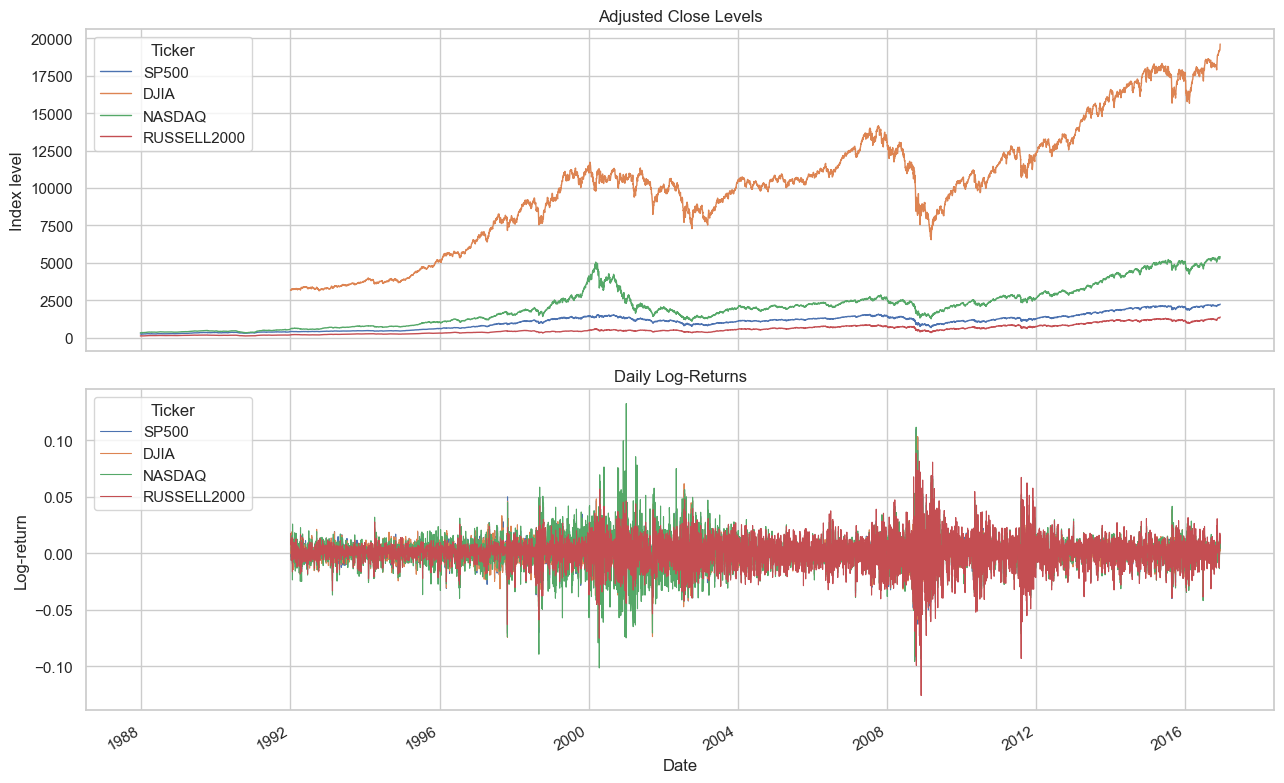
\includegraphics[width=0.9\textwidth]{figures/figure_cell7_out0.png}
    \caption{Preliminary data check from the notebook: adjusted close levels and daily log-returns for the four index series.}
    \label{fig:data_overview}
\end{figure}

\newpage
\section*{Methodologies Implemented}
The methodology follows the original paper's framework with practical implementation decisions in Python:
\begin{enumerate}
    \item \textbf{Rolling point-cloud construction.}  
    For each date, I collect \(w\) consecutive 4D observations (four index log-returns), giving one point cloud in \(\mathbb{R}^4\).
    \item \textbf{Persistent homology computation.}  
    I compute 1D persistence diagrams from each cloud using Vietoris--Rips filtration (via \texttt{ripser}, max dimension \(=1\)).
    \item \textbf{Persistence landscape norm approximation.}  
    I numerically approximate persistence landscapes from birth/death pairs and compute \(L^1\) and \(L^2\) norms for each window.
    \item \textbf{Early warning diagnostics.}  
    On the resulting norm time series, I compute rolling variance and low-frequency spectral power, and apply Mann--Kendall/Kendall-\(\tau\) style trend checks on pre-crash windows.
\end{enumerate}

I am keeping this implementation close to the paper while still using modern Python tools rather than the original R package stack. This should make the replication both transparent and easier to extend later.

\begin{figure}[h!]
    \centering
    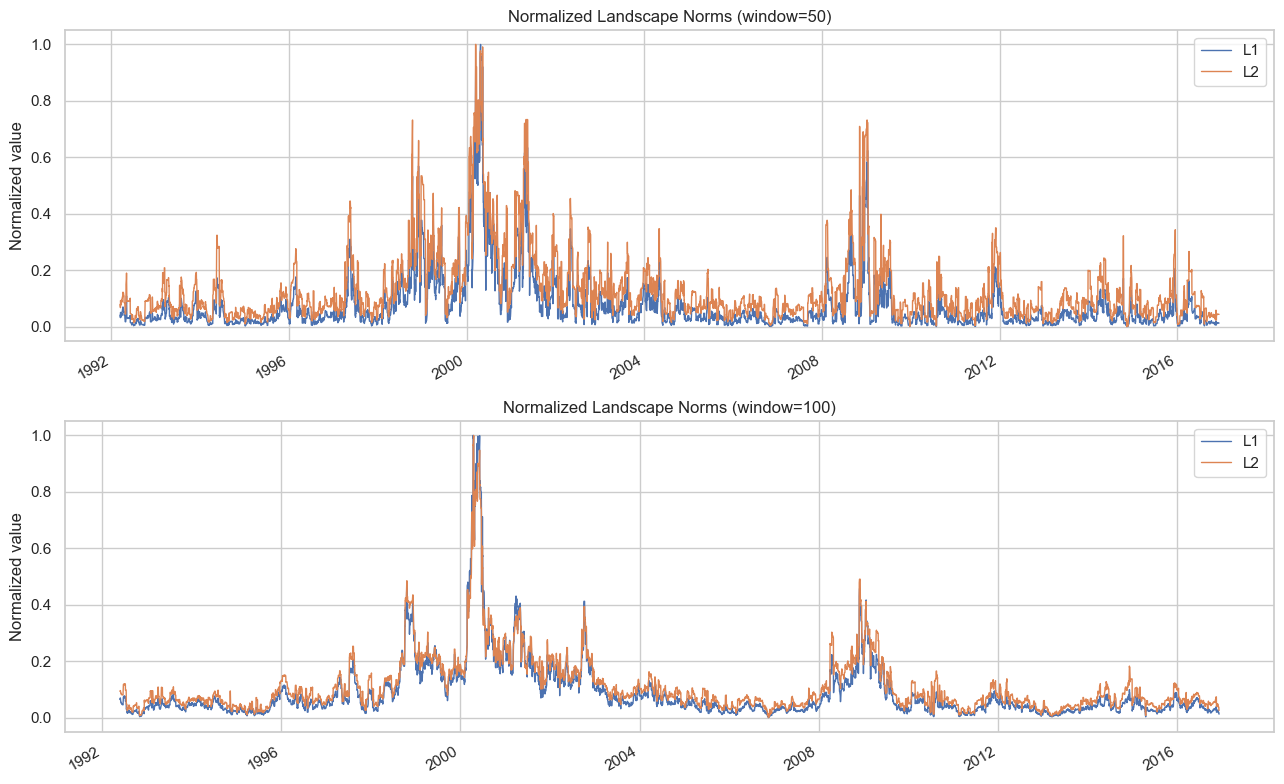
\includegraphics[width=0.88\textwidth]{figures/figure_cell13_out0.png}
    \caption{Normalized persistence landscape norm series (\(L^1\), \(L^2\)) from rolling windows (preliminary replication output).}
    \label{fig:norm_series}
\end{figure}

\newpage
\section*{Expected Results}
Based on current outputs and on the target paper, I expect the final report to show the following:
\begin{itemize}
    \item The time series of persistence landscape norms should increase sharply near major stress periods, with noticeable fore-shocks before the main crash dates.
    \item Rolling variance and low-frequency spectral density of the norm series should exhibit positive trends in the 250 trading days before 03/10/2000 and 09/15/2008.
    \item The topological indicators should provide complementary information to VIX (sometimes sharper, sometimes similar), rather than simply duplicating VIX behavior.
    \item Window size changes (\(w=50\) to \(w=100\)) should preserve the broad signal structure but potentially smooth peaks and shift maxima slightly, as discussed in the paper.
\end{itemize}

In plain terms, I expect to recover the main qualitative claim: TDA-based persistence landscape norms can act as a useful early warning signal class for imminent market crashes. Quantitatively exact figure matching may differ a bit because of implementation details (library differences, numerical approximations, and data vendor updates), but the directional behavior should remain consistent.

\section*{Next Steps}
\begin{itemize}
    \item Finalize figure-by-figure alignment with the paper's event windows and normalization conventions.
    \item Add robustness checks for parameter choices (grid size, filtration effects, and potential scaling sensitivity).
    \item Cleanly document reproducibility details (package versions, run order, runtime notes).
    \item Prepare final write-up linking each reproduced result to the corresponding original figure/claim.
\end{itemize}

\end{document}
